\section{Blokų grandine paremtas tapatybės atributų valdymo modelis}

Atsižvelgus į blokų grandinės savybes, tinkamas tapatybės valdymo problemoms spręsti, šiame skyriuje pateikiamas
blokų grandine paremtas skaitmeninės tapatybės valdymo modelis. Modelis skirtas spręsti ~\ref{IDM:problemsSummarized} skyrelyje
apibendrintoms naudotojų problemoms. Kadangi tapatybės valdymas apima
daug skirtingų procesų, aprašomas modelis apsiriboja asmens tapatybės atributų valdymu ir perdavimu. Kuriamo modelio architektūra 
remiasi MIT tyrime \cite{MITPaper} pristatytais teoriniais protokolais, bandant juos pritaikyti
ne tik mobiliosioms aplikacijoms, o ir interneto tinklalapiams. 

\subsection{Reikalavimai}

Naudotojams kylančios problemos tapatybės valdyme remiasi į tai, kad jų tapatybė yra
visiškai patikėta valdyti tapatybės tiekėjams. Dėl menko naudotojų įsitraukimo į tapatybės valdymo
procesus, asmenys neretai lieka tik pasyvūs stebėtojai.


Siekiant išspręsti šią problemą, kuriamo modelio reikalavimai kurti pagal į naudotoją orientuotos tapatybės
(angl. \textit{user-centric identity}) principus. Ši paradigma akcentuoja naudotojus kaip centrinę
identiteto valdymo sistemų dalį, perduodant paslaugų ir tapatybės tiekėjų turimą tapatybės kontrolę
naudotojams \cite{Cao2010}. Tokiu būdu, naudotojai turi aktyviau prižiūrėti ir dalyvauti tapatybės
valdymo procesuose (dažniausiai naudojant papildomą programinę įrangą),
tačiau geriau žino, kaip ir kur yra naudojami jų asmens duomenys.

Taikant į asmenis orientuotos skaitmeninės tapatybės principus, reikalavimai modeliui suformuluoti naudotojų istorijų forma:

\begin{enumerate}
    \item Kaip interneto naudotojas, aš noriu žinoti, kurios programos turi prieigą prie kurių mano asmens duomenų.
    \item Kaip interneto naudotojas, aš noriu kontroliuoti savo asmens duomenis ir pats suteikti arba atmesti prieigą paslaugų tiekėjams pasiekti mano duomenis.
    \item Kaip interneto naudotojas, aš noriu galimybės lengvai atnaujinti savo asmens duomenis vienoje vietoje.
    \item Kaip interneto naudotojas, aš nenoriu, jog mano asmens duomenų pasiekiamumas priklausytų tik nuo vienos trečiosios šalies pasiekiamumo.
\end{enumerate}

Pateiktos naudotojų istorijos padengia 1 skyriuje apibrėžtus asmenų poreikius tapatybės valdymo
sistemoms bei išskirtas kontrolės, pasitikėjimo ir skaidrumo trūkumo problemas. Saugumo iššūkiai internete
yra plati tema, kuri šiame skyriuje nebus nagrinėjama. \textcolor{red}{ar užtenka tokio sakinio pasakymui kad čia \textit{out of scope}? nes saugumui užtikrint reik
kad naudojamos paslaugos SSL turėtų, ir šiaip plati tema labai, kurios vien blockchain neišspręs}

\subsection{Modelio dalys}

Modelis sudarytas iš dviejų dalių: blokų grandinės (ir joje esančių išmaniųjų kontraktų, aprašančių veikimo logiką)
bei klientinės programos, skirtos naudotojui palengvinti bendravimą (siųsti transakcijas) su blokų grandine ir apžvelgti
autorizuotas paslaugas.

\subsubsection{Blokų grandinė} \label{BCIDM:blockchainFunctions}

Pagrindinė blokų grandinės paskirtis yra pagal išmaniuosiuose kontraktuose aprašytą logiką suteikti arba nesuteikti
prašančioms paslaugoms jų norimus tapatybės atributus. Išmanieji kontraktai yra atsakingi už:

\begin{itemize}
    \item naudotojo atliekamą paslaugų autorizavimą. Naudotojas, kviesdamas išmanaus kontrakto funkciją, gali pasirinkti,
    ar suteikti konkrečiai paslaugai prieigą prie jos norimo atributo. Prieigos yra valdomos ne visos tapatybės, o atributų lygmenyje -
    viena paslauga gali turėti prieigą prie mažiau atributų nei kita.

    \item šifruotų atributų saugojimą. Išmaniuosiuose kontraktuose saugomi naudotojo tapatybės atributai. Jeigu paslaugą P
    naudotojas yra autorizavęs atributui X, tuomet kontrakte išsaugomas P viešu raktu užšifruotas atributas X. Taip tik paslauga P
    su savo viešu raktu galės perskaityti viešajame kontrakte esantį atributą.

    \item pateikiamas funkcijas paslaugoms pasiekti atributus. Išmanusis kontraktas atsižvelgia į tai, kokia paslauga kreipiasi (iš
    jos viešo rakto) bei kokio atributo prašo. Tuomet, patikrinęs, ar ši paslauga turi prieigą, atitinkamai persiunčia
    paslaugai atributą, praneša apie atmestą prieigą arba išsaugo užklausą, laukiančią naudotojo sprendimo.
\end{itemize}

\subsubsection{Klientinė programa}

Klientinė programa yra skirta palengvinti naudotojo bendravimą su blokų grandine. Teoriškai, naudotojas galėtų pats saugoti
savo privatų raktą bei formuoti tiesiogines užklausas į blokų grandinę, tačiau tai nėra patogu. Dėl šios priežasties,
modelyje taip pat pristatoma klientinė programa, kuri stebi (angl. \textit{monitor}) blokų grandinės išmaniųjų kontraktų būseną,
o su šia programa naudotojas gali siųsti pranešimus į blokų grandinę.

Modelyje nėra apibrėžiama, kaip turi būti įgyvendinta ši programa - tai gali būti kompiuterio darbalaukio programa,
mobilioji programėlė ar 
interneto tinklapis. Jos įgyvendinimas būtų panašus į centralizuotos kriptovaliutos piniginės kūrimą (pvz. \enquote{Coinbase}), nes ši
programa skirta palengvinti naudotojo bendravimą su blokų grandine, kuris aprašytas~\ref{BCIDM:blockchainFunctions} skyrelyje.

Klientinė programa saugo naudotojo privatų raktą, praneša apie naujas paslaugų užklausas, padeda šifruoti
į blokų grandinę saugomus atributus su paslaugos viešuoju raktu.

\subsection{Naudojimo sekos}

Šiame skyriuje UMl sekų diagramomis pateikiami pagrindiniai modelio panaudos atvejai (angl. \textit{use cases}).

\subsubsection{Naudotojo viešo rakto suteikimas paslaugai}

Kai naudotojas pirmą kartą pasinaudoja paslauga, paslauga paprašo naudotojo pateikti jo viešą raktą. Taip paslauga
su šiuo raktu galės kreiptis į blokų grandinę ir atlikti pageidaujamų atributų užklausas.

\begin{figure}[H]
    \centering
    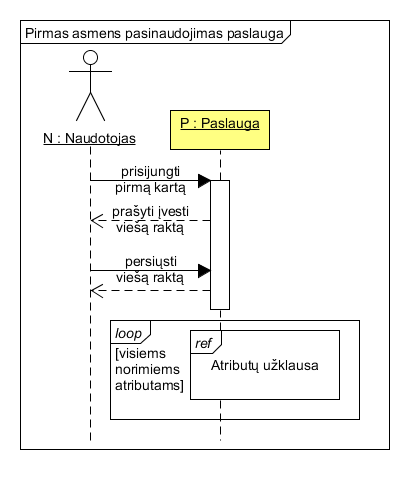
\includegraphics[scale=0.8]{img/initiateUserServiceRelationship}
    \caption{Pirmas naudotojo pasinaudojimas paslauga}
    \label{fig:initiateUserServiceRelations}
\end{figure}

\subsubsection{Paslaugos atliekama atributo užklausa}

Aprašymas.

\begin{figure}[H]
    \centering
    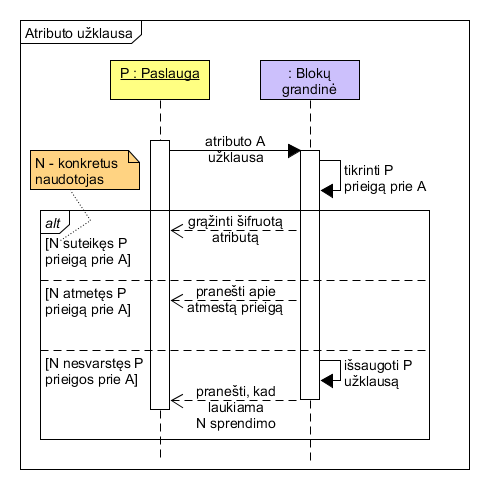
\includegraphics[scale=0.8]{img/askForAttributeSequence}
    \caption{Pirmas naudotojo pasinaudojimas paslauga}
    \label{fig:askForAttributeSequence}
\end{figure}

\subsubsection{Naudotojo atliekamas paslaugos autorizavimas}

Aprašymas.

\begin{figure}[H]
    \centering
    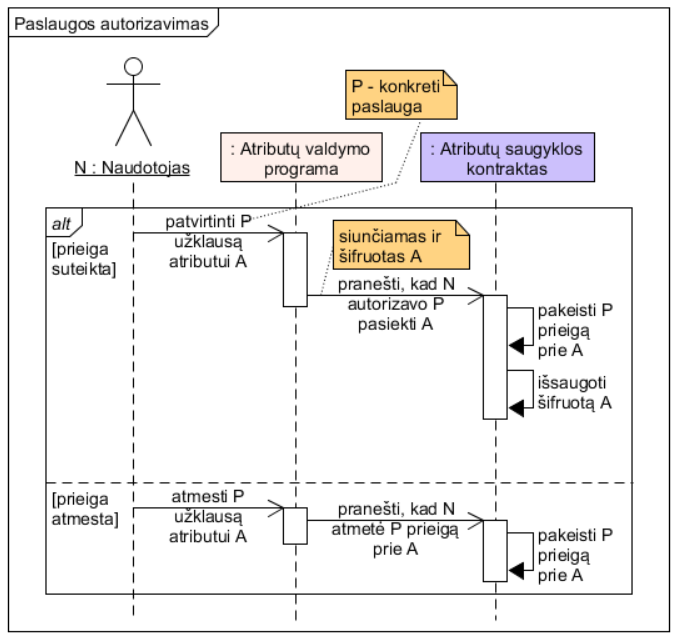
\includegraphics[scale=0.8]{img/givePermissions}
    \caption{Pirmas naudotojo pasinaudojimas paslauga}
    \label{fig:givePermissions}
\end{figure}

\subsubsection{Klientinės programos atliekamas blokų grandinės stebėjimas}

Aprašymas.

\begin{figure}[H]
    \centering
    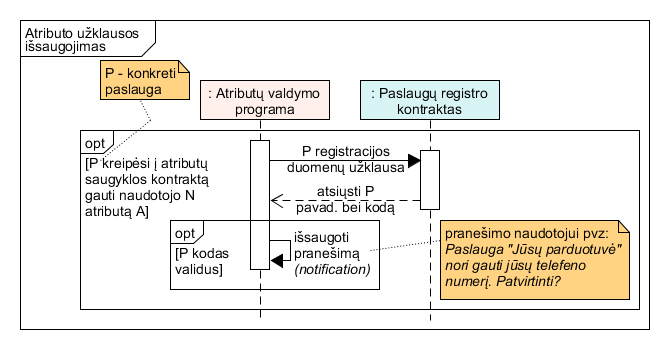
\includegraphics[scale=0.8]{img/checkForPendingPermissions}
    \caption{Pirmas naudotojo pasinaudojimas paslauga}
    \label{fig:checkForPendingPermissions}
\end{figure}